\documentclass[12pt,a4paper]{article}
\usepackage[margin=1.2in]{geometry}
\usepackage{times}
\usepackage{graphics}
\usepackage{graphicx}
\usepackage[sort&compress]{natbib}
\usepackage{durhampaper}
\usepackage{subcaption}
\usepackage{caption}
\usepackage{todonotes}
\usepackage{times} 
\usepackage{wrapfig}
\usepackage{glossaries}
\usepackage{setspace}
\usepackage{booktabs}
\usepackage{enumerate}
\usepackage[compact]{titlesec}
\usepackage[font=small,labelfont=bf, textfont=it]{caption}
% \usepackage{harvard}
\usepackage[moderate]{savetrees}
\usepackage{url}
\usepackage{microtype}
\usepackage{amsmath}
\usepackage{multicol}

\makeglossaries
\title{Facial Liveness Testing: an approach for the web}
\author{} % leave; your name goes into \student{}
\student{Ryan Collins}
\supervisor{Prof A. Krokhin}
\degree{MEng Computer Science}
\def\bibfont{\footnotesize}
\setlength{\bibsep}{0.4ex}
% \renewcommand{\baselinestretch}{0.87}
\setlength{\textfloatsep}{2pt}
\date{\today}
\titleformat{\section}
{\normalfont\Large\bfseries}{\thesection}{1em}{}
\titleformat{\subsection}
{\normalfont\large\bfseries}{\thesubsection}{1em}{}
\titleformat{\subsubsection}
{\normalfont\normalsize\bfseries}{\thesubsubsection}{1em}{}
% Now the main body of the document.
\begin{document}
\maketitle
\begin{abstract}
% These instructions give you guidelines for preparing the final paper.  DO NOT change any settings, such as margins and font sizes.  Just use this as a template and modify the contents into your final paper.  Do not cite references in the abstract.
% However, with facial recognition comes face spoofing: methods to fool the algorithms into thinking one is someone different to who they are.
% The abstract must be a Structured Abstract with the headings {\bf Context/Background}, {\bf Aims}, {\bf Method}, {\bf Results}, and {\bf Conclusions}.  This section should not be longer than half of a page, and having no more than one or two sentences under each heading is advised.
\paragraph{Context}
    Existing password-based authentication systems are insecure, being susceptible to many different types of attacks. One proposed solution has been face recognition, but with this new authentication method comes a problem:
    how can spoofing be stopped. Liveness tests, a method for detecting when spoofing has occurred within the image, are the solution. With newer, real-time liveness tests, face recognition systems can become more secure and
    hopefully more mainstream. The liveness tests of the future require a standardized input, which can use existing hardware. Furthermore, these liveness tests need to be fast to execute. In addition, a module is needed to allow multiple liveness tests to work together to yield a single liveness value.

    This project developed several new liveness tests to meet these requirements. A module to fuse liveness tests together is also produced, with more testing on more liveness tests required.

\paragraph{Aims}
    % This might belong more in the method.
    The aim was to develop three liveness tests: one to predict liveness based on image quality, one to use facial structure and texture as a liveness measure,
    and a final one to predict 3D liveness attacks (specifically mask attacks). Each of these metrics were required to classify liveness for a single image within a maximum of 2 seconds.
    Furthermore, no special hardware was allowed, to ensure these liveness tests can be used by as many people as possible through mobile devices/laptop computers.
    The aim was also to combine the results of these liveness tests together in some consolidation layer, providing a single definitive liveness value.
\paragraph{Method}
    This project involved the design, training, and testing of three different innovative liveness tests. The NUAA and Replay-Attack devel datasets were used for training, with the Replay-Attack test dataset being used for testing.
    
    The first test developed was the Whole Image Quality Assessment (W-IQA) liveness test which analysed image quality across the entire image, using a combination of 24 different image quality metrics with a Linear Discriminant Analysis classifier (LDA) to predict liveness.

    The second test developed was the Convolutional Neural Network (CNN) based 2D liveness test, which utilised a pre-existing image classification model and adapted it to the role of facial liveness testing.

    The third was a 3D based liveness test to detect mask attacks. This process combined existing techniques for reconstructing a face in 3D from a 2D image, and fed this reconstruction through a VoxNet classifier to detect whether the 3D data contained spoofed input or real input.

    Using the classification probabilities from liveness tests, an LDA based classifier was then trained to fuse the results of the above metrics together, to improve accuracy and allow for future expansion with further liveness tests.
  
\paragraph{Results}
    2D attacks were tested using the Replay Attack test dataset. Top-1 accuracy was measured to determine overall performance. 

    The W-IQA test performed admirably, producing an 87\% accuracy. When this test produced errors, false positives were more common which led to spoofed images being classed as real.

    The CNN based 2D liveness test performed adequately, yielding a 71\% top-1 accuracy. When this test produced errors, false negatives were far more common which yielded fewer security concerns.

    The 3D based liveness test performed poorly due to a long reconstruction time (5 seconds), coupled with incredibly high memory usage.

    A consolidation layer was designed, based on the LDA classifier, and this yielded similar accuracy statistics to the above liveness tests.
\paragraph{Conclusions}
    W-IQA and 2D CNN liveness tests showed promising results for inclusion in a real-time liveness system. Prediction time for both tests was within a 2-second limit. Both tests required no special hardware.

    The W-IQA test produced excellent accuracy scores but was let down by false classification of spoofed images as real. Resolution differences also led to performance problems. This model would be improved by utilizing data with different resolutions.

    The 2D CNN test produced satisfactory accuracy scores but showed impressive caution at classifying faces correctly. Future work should improve the datasets used, to guarantee each image has a detectable face.

    The 3D mask attack detection test performed poorly due to tremendous memory requirements. 2D to 3D reconstruction time also took longer than the required time for a single prediction. This liveness test is not suitable for real-time liveness prediction.

    The consolidation layer produced worked well, but needs to be tested with a larger number of liveness tests to confirm it's the most ideal solution to the problem.
\end{abstract}

\begin{keywords}
Facial liveness, convolutional neural networks, image quality metrics, residual networks, anti-spoofing
\end{keywords}

\section{Introduction}
    Facial recognition is becoming an increasingly popular method for authentication. However, these methods still have opponents. Adam Schwartz, a lawyer with the Electronic Frontier Foundation,  criticized these methods by saying "We can change our bank account numbers, we can even change our names, but we cannot change our faces.
    And once the information is out there, it could be misused". \cite{NPRArticle}

    For facial recognition to become more widespread, methods of detecting spoofing are necessary, to ensure stolen identities can't easily yield security problems. Liveness systems are the answer to this problem. 

    While different methods of detecting liveness are available, these are specialized towards defending against a different type of attack.
    Some existing liveness tests require the use of specialized hardware or sensor configurations that are not available in most smartphones/computers. 
    This work aimed to develop liveness tests requiring a single camera as input. The proposed liveness tests were required to produce predictions in near-real time (2 seconds) with sufficient accuracy.
    This work also proposed a method of fusing liveness test results to produce an absolute liveness value, for use within recognition applications.
    Future extensions could apply the tests proposed here for applications within web-based or internet of things (IoT) applications. 

    Therefore, the objectives of this project could be summarised by the following:

    \begin{center}
        \begin{enumerate}
            \item Build, train, and test an image quality based liveness test
            \item Build, train and test a Convolutional Neural Network liveness test
            \item Build, train and test a liveness test to detect 3D mask attacks
            \item Design and test a method for fusing liveness test results together, to produce a definitive liveness measure
            \item Assess the created liveness tests for real time performance characteristics, to ensure they can run in real-time.
        \end{enumerate}
    \end{center}

    In this context, a new 2D CNN based liveness test was proposed, used to analyze 2D facial images for liveness. An existing quality-based test was also modified to provide liveness scoring based on image quality. For 3D based mask attacks, a new liveness test was also developed based on a 2 part approach: (i) VRN based 3D reconstruction (ii) VoxNet based 3D classification.
    An LDA based consolidation layer was constructed to fuse liveness test results together, which yielded positive results but requires further testing.
\section{Related Work}
    As defined in \cite{FaceSpoofingAttacksStudy}, there are three common types of spoofing attack: Photo Attack, Video Attack, and Mask Attack.
    Photo and Video attacks are both classed as 2D spoofing attacks, while mask attacks are 3D attacks.

    \subsection{2D Spoofing Attacks}
        2D based attacks rely on presenting a previously retrieved photo/video, on some medium, to the camera input. Photo attacks rely on a single printed photo being presented. Video attacks consist of a video being played back on a screen. \cite{FaceSpoofingAttacksStudy}
        
        The different methods of liveness tests are shown the the following sections.

        \subsubsection{Video-based tests}
        Since video consists of multiple frames, motion can be used to determine liveness. 

        \paragraph{Depth-based liveness}

        The method proposed in \cite{SFMClassifier} uses a structure from motion (SFM) process to reconstruct a person's face in 3D and uses depth information to consider whether the person is real. The process then extended this by fusing depth information with audio verification to improve the prediction results, using a Bayesian network. \cite{SFMClassifier} While this worked with large amounts of motion, running SFM on a video with little motion yields a result with little depth. Another drawback was the requirement for video input since video capture is more time consuming and more challenging.
        
        \paragraph{Blink Detection}
        The blink detection test analyses natural video input to determine whether blinking has occurred. Unlike other video-based methods, this looks for natural behavior rather meaning the user isn't required to carry out any motion. \cite{BlinkDetectionLivenessTest} 
        However, this test can be easily defeated by making eye holes within a printed picture. 
        Furthermore, investigating this liveness method is difficult due to the shortage of video data available.
    
        % Face Flashing
        \paragraph{Face Flashing}
        Possibly the most promising video-based liveness detection test, this method relies on a screen acting as a light source and considering the color and reflective properties of light. Light reflects differently off a face compared to a piece of paper/mask, and therefore the light reflections can give an indication into liveness. Different colors can also be used to add an element of randomness, requiring specific color patterns to be detected. Flashes also occur with different temporal patterns, yielding an additional expected metric.

        While incredibly promising, this method requires the use of a screen. While screens are a common component in smartphones and computers, they are less commonplace in some IoT devices. 

        Furthermore, testing this method would be difficult, as existing datasets don't contain any flashing information required. 

        However, in the future, this method could be implemented to add further security into a facial liveness system on the web, where video input is available.
        
        \subsubsection{Quality-based tests}
        When presenting another medium to a camera, there will be a loss in the resultant image, since printers can't replicate all details, and neither can screens. Therefore, by measuring the image quality of an input image, one could train a classifier to predict liveness.

        One existing method utilized this premise by using the result of 25 different image quality metrics to classify realness using a Linear Discriminant Analysis (LDA) classifier. The results were impressive, 
        yielding very little error (3\% on the iris dataset, no error was given for the facial liveness attempt). The overall method was applied to multiple different types of biometric data, but with facial information the facial data was used, containing very little background information. \cite{ImageQualityAssessmentTest}
        By adding background information, it might be possible to detect further quality differences elsewhere. 
        
        Overall, there is a benefit of fusing results together using a classifier. This same method could be adapted to combine the results of multiple liveness tests together.

        % Several different existing networks exist.
        % However, work in this space could be improved, and to do this an understanding of the models is required.

        \subsubsection{Neural Networks, and their structure}
        Developing a custom deep learning model requires an understanding of deep neural networks. These consist of many different layers, each linked by weights. Deeper neural networks have recently allowed for more accurate models. Therefore, an understanding of layers is vital.

        \paragraph{Fully connected layers} Fully connected (or dense) layers consist of neurones. Given two layers $l_1$ and $l_2$, each
        neuron $n_i$ in $l_1$ is linked to each neuron $n_j$ in $l_2$ with a weight $w_{i, j}$. For each neuron in the previous layer, the output of that neuron is multiplied by a weight, the total is summed,
        and the sum is put through a function $t(x)$ which is the activation function. Examples of activation functions include \emph{reLU}, \emph{sigmoid}, and \emph{hyperbolic tangent}.
        $$n_j = t(\sum_{i \in PrevLayer}(n_i * w_{i, j}))$$

        \paragraph{Convolutional layers} Designed primarily for images, these convolve over an image with a kernel. For each location over an image, the weights are multiplied by the image input at that particular location. These are then fed through an activation function.
        The output of a convolutional layer would be a multidimensional tensor. While 2D images are primarily used for input, 3D convolutional layers follow this same process for 3D representations. 
        Convolutional layers are better suited for images compared to fully connected layers, since fewer weights (also known as parameters) are required, thus reducing the required computation and storage. I believe CNNs provide a key approach to facial liveness since they can be used to learn a variety of features including face structure,
        texture, and other potentially suspicious visual glitches which would be obtained with face spoofing.

        \paragraph{A note about parameters}
        Parameters are a measure for how complex a network is, and therefore how difficult training and prediction is. It's an indication of how large the model needs to be. Parameters define how many connections exist within the neural network.

        \paragraph{Cross-Database Approach}
        While using one dataset can be suitable, using multiple datasets can allow a model to be better at predictions on unseen data (better at generalising). This is the method used in \cite{Patel2016CrossDatabaseFA}, which utilises multiple datasets to improve the amount of training data available, and to provide a completely independent test dataset.
        This method also fuses multiple methods together, to further analyse quality using a CNN, ensuring the features can be
        more easily learned. The drawback with this method however is the large amount of convolutional layers that are required. 
        
        \subsubsection{General 2D image classification models}
        The process of facial liveness can be considered an image classification problem. 
        While previous works have focused on developing new methods to solve the liveness problem, a prudent approach might be to apply an existing image classification model to the problem. 
        Recent research into visual object recognition has led to the development of different neural network architectures, which have gained excellent results in solving this problem.
        Many of these architectures also operate with reasonable computational requirements.
        These models use a dataset called the ImageNet dataset, which contains images separated into 20,000 categories. However, some variations exist with fewer categories.
        These different models include:
            
            \paragraph{AlexNet} 
            This model contains 5 convolutional layers and 2 fully-connected layers, with additional max-pooling layers to reduce dimensionality. 
            This model was used to classify 1.3 million high-resolution images into 1000 classes. \cite{AlexNet} 
            With a low number of parameters, AlexNet is fairly easily deployed (since fewer computation resources are required). Figure \ref{Top1AccuracyOverOperations}
            shows that AlexNet requires very few operations, in the range of $<10$ G-Ops. 
            One drawback to AlexNet is the functionality: top-1 classification accuracy isn't as high as more recent methods. As a result, this isn't the most suitable model to use.
            \cite{DeepNeuralNetworkDeployability}
            
            \paragraph{VGG16 Network}
            VGG consists of blocks containing two convolutional layers with fewer filters, and a max pooling layer.  This yields greater liveness prediction results as opposed to AlexNet but requires far more processing power.
            In total, VGG contains 128 million parameters (weights), therefore requiring a large amount of memory and processing power to train, and make a single prediction. 
            \cite{DeepNeuralNetworkDeployability} 
            
            Due to these high computational requirements, this model isn't the most suitable for a real-time system.

            \paragraph{GoogLeNet Inception}
            
            GoogLeNet is an improved module that approximates a space Convolutional Network with a feed-forward construction. One of the major features of GoogLeNet is the Inception module.
            Naively, this inception module requires input from the previous layer, and calculates a 1x1, 3x3 and 5x5 convolution simultaneously, along with a 3x3 max pooling, before feeding all of these outputs into the filter concatenation step. 
            This naive implementation isn't as efficient. Efficiency can be improved by reducing dimensionality. The solution is to apply a 1x1 convolution before each 3x3 and 5x5 convolution, after the max-pooling output. 
            These inception modules can be used and stacked to improve performance without a huge increase in computation. \cite{GoogLeNet} 
            
            Comparatively, GoogLeNet produces improved top-1 accuracy scores compared to AlexNet, as shown in Figure \ref{Top1AccuracyOverNetwork}. 
            GoogLeNet also produces similar results to the VGG model.

            There have been several different version of GoogLeNet. Analyzing the data shown in Figure \ref{Top1AccuracyOverOperations}, more recent versions 
            have yielded improved accuracy characteristics; the Inception-4 model produced the best accuracy scores out of all the ImageNet classifiers. However, 
            this improved accuracy increases the number of operations required. Older versions of GoogLeNet required $<10$ G-Ops, while Inception v-4 required $~18$ G-Ops.
            Compared to VGG, this model performs well, but Residual Network models arguably provide a better balance between accuracy and computational requirements.
            \begin{wrapfigure}{l}{200px}
                \centering
                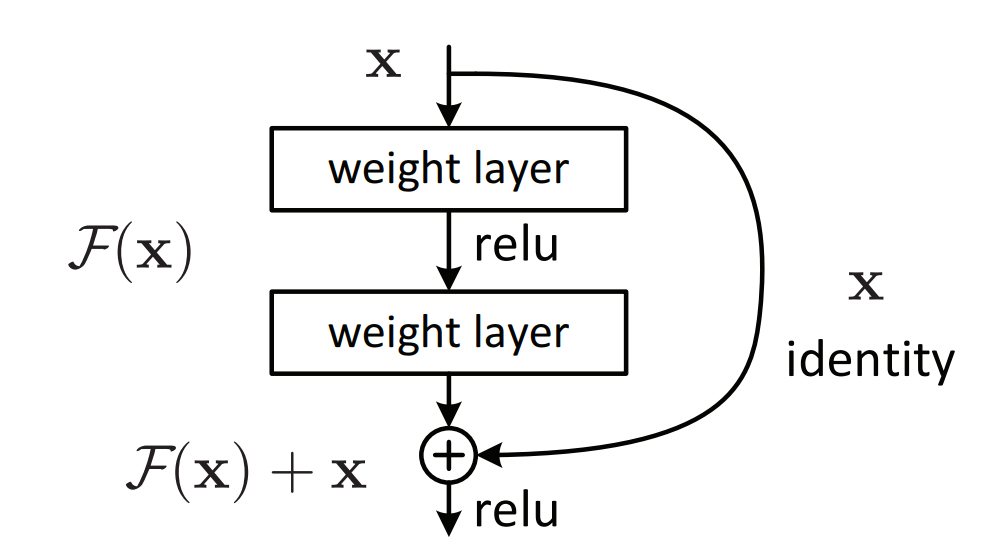
\includegraphics[width=200px]{ResidualBlock.png}
                \caption{A Residual Block: this is the building block of the ResNet architecture. Source: \cite{DeepResidualNetworks}}
                \label{ResidualBlock}
            \end{wrapfigure}
            \paragraph{Residual Networks}
            Residual Networks (ResNets) aim to improve traditional convolutional networks by reducing the vanishing gradient problem, therefore decreasing training time.
            This problem occurs when early layers have a small gradient, which yields even smaller gradients during later layers. 

            Residual blocks, shown in Figure \ref{ResidualBlock}, solve this problem by utilizing shortcut connections during training, allowing gradients to skip layers if necessary. 
            These connectors work by adding their outputs to the stacked layers.

            Figure \ref{Top1AccuracyOverNetwork} shows that this method yields better accuracy than both VGG and GoogLeNet. In terms of computational performance, 
            Figure \ref{Top1AccuracyOverOperations} shows that ResNet50 requires fewer than 10 G-Ops, whilst yielding 76\% accuracy.

           

            \begin{figure}
                \centering
                \begin{subfigure}[t]{.4\textwidth}
                    \centering
                    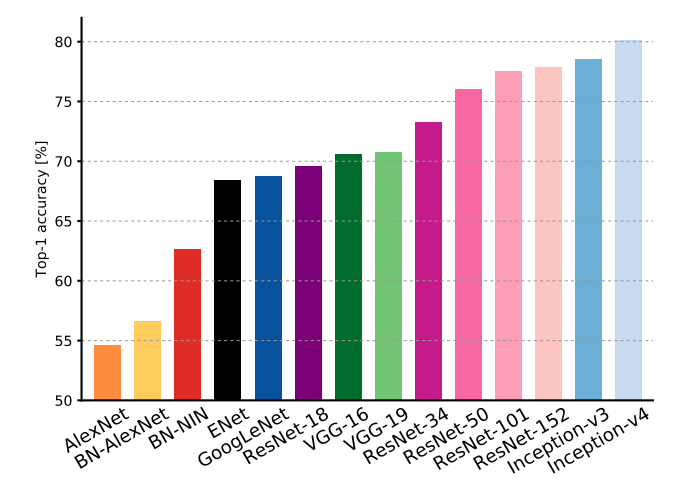
\includegraphics[width=\linewidth]{Top1AccuracyOverNetwork.png}
                    \caption{Top 1 accuracy vs network. Chart and results from \cite{DeepNeuralNetworkDeployability}}
                    \label{Top1AccuracyOverNetwork}
                \end{subfigure}
                \hfill
                \begin{subfigure}[t]{.4\textwidth}
                    \centering
                    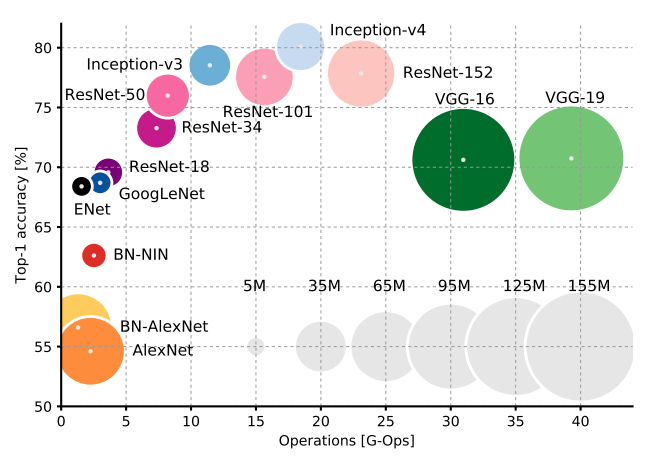
\includegraphics[width=\linewidth]{Top1AccuracyOverOperations.png}
                    \caption{Top 1 accuracy vs operations, where network size is proportional to number of parameters. Operations figures are for a single pass (e.g. predicting given a specific input). Chart and results from \cite{DeepNeuralNetworkDeployability}}
                    \label{Top1AccuracyOverOperations}
                \end{subfigure}
                \label{ComparisonsOfDifferentModels}
                \caption{These two charts, from \cite{DeepNeuralNetworkDeployability}, show the accuracy and computational requirements of each type of classifier.}
        \end{figure}

        \subsubsection{Datasets}
        %Datasets
        One of the earliest datasets available for facial liveness was the NUAA dataset. This contained photographs of 15 different subjects, both real and fake images.
         Spoofed images were of paper replay attacks, with the displayed images being both warped and flat. 
         The dataset contained JPEG images with a hierarchical structure. One drawback with this dataset is licensing: the dataset is only available for non-commercial use, 
         such as research purposes. Future, more commercial works, would, therefore, require a different dataset be used in order to meet the licensing objectives. \cite{NUAADataset}

        In 2012, the Replay-Attack dataset was first released, consisting of 1,300 video clips. These video clips contain both real and spoofed data. Spoofed data contains a mixture of different attack methods,
        including printed photograph, video, with both high and low-resolution media. To facilitate training, testing, and validation, the dataset also contains sub-datasets.
        The 'devel' dataset was designed for training and validation purposes, while the 'test' dataset was designed for testing the trained model.  \cite{ReplayAttackDataset}

        While individually, these datasets might not contain enough data, together they provide enough samples to reasonably train and test our models.
        They shall be used throughout this project for both training and testing the 2D based liveness models.

            
    \subsection{3D Spoofing Attacks}
       
        Mask Attacks are a 3D spoofing attack, which involves creating a 3D mask of someone and wearing it. \cite{FaceSpoofingAttacksStudy}
        While these are currently much less prevalent, the improvement in 3D printing technologies could lead to this becoming more common in the future.

        \subsection{Dataset}
        Released in 2013, the 3D Mask Attack Dataset (MAD dataset) contains 76500 frames of 17 people, recorded using an Xbox Kinect camera.
        Each frame contained a depth image, a 2D RGB image with 8-bit color and a size of 640x480 pixels. Each frame also contained eye positions.
        All data samples were stored in an h5 file. The first two sessions contained occurrences of real accesses, while the third session contained data relating to attacks.
        The filename also contained information regarding the subject present in the set of images. 
        
        \cite{3DMadDataset}

        \subsubsection{Obtaining 3D data from 2D images/video}
            
            \paragraph{Structure from Motion (SFM)}
            A well-known 2D to 3D conversion method, SFM obtained depth data from movement available within multiple images (a video). Depth is obtained by utilising a calibrated camera and conducting point matches between images
            to determine an appropriate transform to world-space. This method was used previously in \cite{SFMClassifier} to consider depth information for 2D based attacks to much success.
            However, when presented with a small amount of motion, depth information would be harder to obtain. Furthermore, since this requires a video input, this would not work as a single image liveness test. Therefore, SFM isn't as useful for this project.
            
            \paragraph{Single Image 3D Face Reconstruction (VRN)}
            \begin{wrapfigure}{r}{150px}
                \centering
                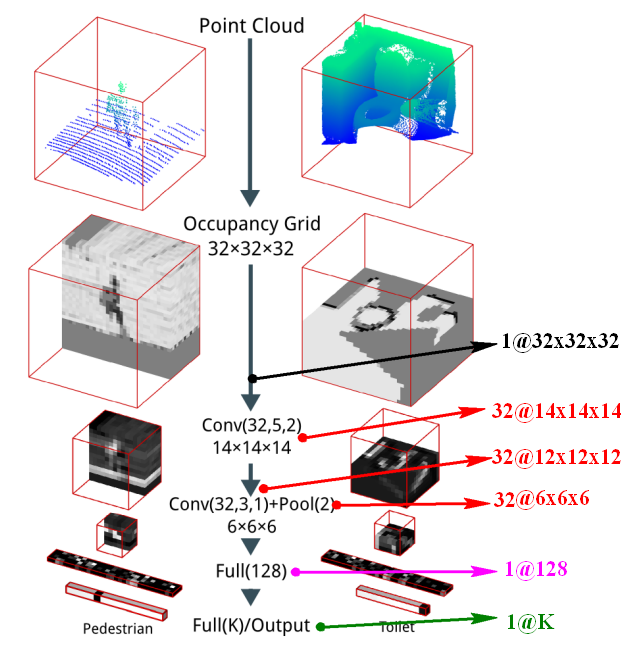
\includegraphics[width=150px]{VoxNetArchitecture.png}
                \caption{The original VoxNet architecture. While point cloud input is available, voxel based representation can also be used. Diagram obtained from \cite{VoxNetModel}}
                \label{OriginalVoxNetArchitecture}
            \end{wrapfigure}
            The method proposed in \cite{3DReconstructionMethod} produces a 3D model from a single 2D image. The model utilizes a pre-trained neural network, implemented in Torch, which turns a 192x192 sized image into a voxel-based representation.
            This model appears suitable for our purposes since it requires only a 2D image rather than a video. Another benefit is the reduced amount of input required from the user. Figure \ref{3DReconstructionScreenshot} shows an example of a 3D facial reconstruction. 
            This screenshot was obtained from the Keras port (since this is more suitable for our project).
            

        \subsubsection{3D Classifiers}
            

            In a similar approach to the 2D methods researched above, there are a variety of existing 3D classifiers that could be re-purposed for the liveness classification approach.
            While these methods don't yield the same accuracy figures as with ImageNet, further improvements in the field of 3D classification could lead to better liveness methods in the future.
         
            \paragraph{PointNet}
            PointNet is a model for classifying point clouds, represented as an unordered set of points. This model has a total of 3.5 million parameters, yielding 440 million operations per sample. 
            While this is still rather high, it's a reasonable number of 3D-based classifiers. This network relies on a sparse input, given as a point cloud, and utilizes a feed-forward network to classify the input.
            Performance is slightly better than VoxNet, with slightly improved computational performance, but both elements don't yield massive differences. \cite{PointNet}
            
           
            \paragraph{VoxNet}
            
            VoxNet requires a voxel representation as input. While point clouds and voxels are equivalent, utilizing this model with the VRN reconstruction method would require less data augmentation. Accuracy of this model isn't that great, yielding 72\% accuracy on the SUOD dataset. \cite{VoxNetModel} However, when investigating this model personally, an accuracy of 68\% was obtained, using the SUOD dataset. 

            The model itself was developed to identify objects based on their 3D representation, which is fairly similar to the ImageNet models from before, only in 3D instead of 2D. 
            Figure \ref{OriginalVoxNetArchitecture} shows the architecture of this classifier. 3D convolutional layers are used to learn the 3D feature space, with a feed-forward layer
            being used to produce the prediction (either of which object has been detected, or whether a spoofed image or real image has been detected).

            While not necessarily being the best model for the job, this provides an ideal proof of concept to this liveness test.
             

\section{Solution}
    % Solution to the problem
    \subsection{Specification, and design requirements}
        \begin{enumerate}
            \item \label{SpecPoint1} Any liveness test produced must be able to predict a single image in under 2 seconds on a standard i7-7700k powered machine
            \item \label{SpecPoint2} Any liveness test must only require the use of a 2D image input from a standard built in camera. No other external hardware is allowed.
            \item \label{SpecPoint3} The Top-1 accuracy figure of each liveness test should be greater than 70\%.
            \item \label{SpecPoint4} The liveness test consolidation layer must allow for future inclusion of further liveness tests.
            \item \label{SpecPoint5} A liveness test should be developed to classify the entire image, to detect spoofing given a specific input.
            \item \label{SpecPoint6} A liveness test should be developed to detect liveness based on the 2D input of a facial area from a camera.
            \item \label{SpecPoint7} A liveness test should be developed to specifically detect 3D based attacks (mask attacks).
        \end{enumerate}

        \ref{SpecPoint1} was important to ensure that the liveness tests that are built didn't take too long to execute and yield a result. While in practice an Intel i7-7700k machine might possess a
        slightly higher clock speed than a standard cloud-based processor, the results yielded would still be reasonable in practice since it acts as a benchmark to compare against.

        Some of the liveness tests proposed in previous works require the use of specialized hardware which won't be available on many devices. The most common device capable of taking in facial input is a
        webcam, and since these are found in many laptops, IoT devices, and smartphones, this is an ideal limiting factor. While screens could also be considered useful, certain IoT devices might not necessarily have them either.
        This is what \ref{SpecPoint2} aims to address.

        The results of the liveness tests produced are also important, since a random prediction of liveness yields a 50\% accuracy, so, therefore, a 70\% accuracy yields a reasonable performance over this, and might require extension to improve it further,
        while a higher accuracy indicates that the liveness test performs better and might have been refined more. This is what \ref{SpecPoint4} addresses.

        \ref{SpecPoint5}, \ref{SpecPoint6} and \ref{SpecPoint7} propose the required features that are used for each liveness test. Whole image detection is necessary to allow a liveness value to be produced even if no face is found through facial extraction methods. Facial structure and texture is necessary since this features isn't covered by a quality metric and could yield better results where quality is hard to distinguish. Finally, a method of predicting mask attacks would be ideal, since 3D attacks could become more common in the future with recent developments in 3D printing technology.

        With these specifications in mind, the design focused on three different liveness tests: an Image Quality assessment based liveness test, a ResNet 50 based classifier (based on a pre-trained ImageNet model),
        and a novel 3D based classifier using 3D facial reconstruction models interlinked with the VoxNet 3D classification model.


    \subsection{Shared Services}
        Each liveness test, and the training and testing process, required some shared subroutines and functions. This section outlines these, and how they were designed and built.
        \subsubsection{Dataset Managers}
        Dataset managers were required to read datasets, and to load them into memory. Programmatically, an abstract class was created to represent an abstract dataset, containing functions to read the dataset and conduct any necessary preprocessing. This class was then extended by implementing dataset managers for the NUAA, Replay-Attack, and Mask-Attack datasets. This generic implementation allowed for datasets to be easily added, providing a class definition as an implementation guideline. 

        On the lower level, a dataset manager was designed to load a dataset from a folder structure, conduct any basic preprocessing to convert the files and their representations into OpenCV based images, and produce a single H5py file containing two datasets: one for spoofed images, and one for real images. H5py was used to produce a single normalized format between datasets which otherwise varied massively in structure. The use of H5Py also reduced the amount of main memory utilized, by caching images on the hard disk and only loading into main memory when required. This was a far more efficient method compared to loading an entire dataset into RAM at once.

        \subsubsection{Neural Network Infrastructure}
            % Keras to simplify models, tensorflow as the underlying backend.
            % Training machine on Google Cloud, using 64GB RAM, 8 x vCPUs, and an NVIDIA Tesla P100 GPU to improve performance of the training process through parallelism. 
            While neural networks can be implemented from scratch, libraries were necessary to reduce the amount of code needed and to improve performance of the models fetched.
            Furthermore, specific hardware was necessary to train and test all models, and these details are outlined in this section.

            \paragraph{Neural Network Framework} 
            Where neural networks were necessary, Keras was used to provide a high-level interface to create, train and test new models. A high-level interface was chosen to allow for easy modification of models and to allow for portability since backends could be changed in the future if necessary without requiring a complete code rewrite.

            A backend was necessary, and therefore Tensorflow was chosen due to a large amount of support available, coupled with the ease of switching between GPU and CPU training. During the model creation process, the \emph{tensorflow} package was used to provide CPU based training. Once a model was to be properly tested, \emph{tensorflow-gpu} was used to train on GPU, reducing training time through parallelism.  

            \paragraph{Hardware for training}
            Training the neural network required more processing power than was directly available. Google Cloud Compute Engine was used to provide this processing power since it was easily accessible and had existing deep learning environments with Intel-accelerated mathematics libraries. 
            The Google Cloud instance also provided easy extensibility, since some of the liveness tests required additional tools that could not be easily installed on NCC/Hamilton clusters at Durham University. The training was conducted on a virtual machine with 64GB RAM, 8 virtual CPUs
            with an NVIDIA Tesla P100 GPU being used to accelerate the training process (through parallelism).

            \paragraph{Hardware for testing}
            GPUs are expensive, and therefore if such a system were deployed the cost of GPUs would provide expensive to run. Therefore, a CPU-only implementation for the testing was followed, using an Intel i7-7700K (at 4.2 GHz), with 16GB RAM, and a SATA SSD. Performance metrics were yielded using this hardware to emulate the expected performance and understand which metrics performed best and whether they performed adequately.

        \subsubsection{Image Processing and Computation Management}
            OpenCV was used to manage the processing of images, including the image loading components. This library was chosen for the wide support available, and for the large feature set that it provides (including Gaussian Blurring, some image metrics, and some Fourier analysis).
            For the rare occasions where OpenCV didn't have the required functionality, scikit-image provided some operations that were necessary.
            
            Numpy was instrumental in most other computation operations (including image preprocessing, mathematical calculations), due to the large speed improvements provided by the C implementation (compared to Python's slower math libraries).
            Since OpenCV interfaces well with Numpy, no conversion was needed which improved the ease of implementation.

        \subsection{Image Quality Assessment Liveness Test}
           \begin{figure}
                \centering
                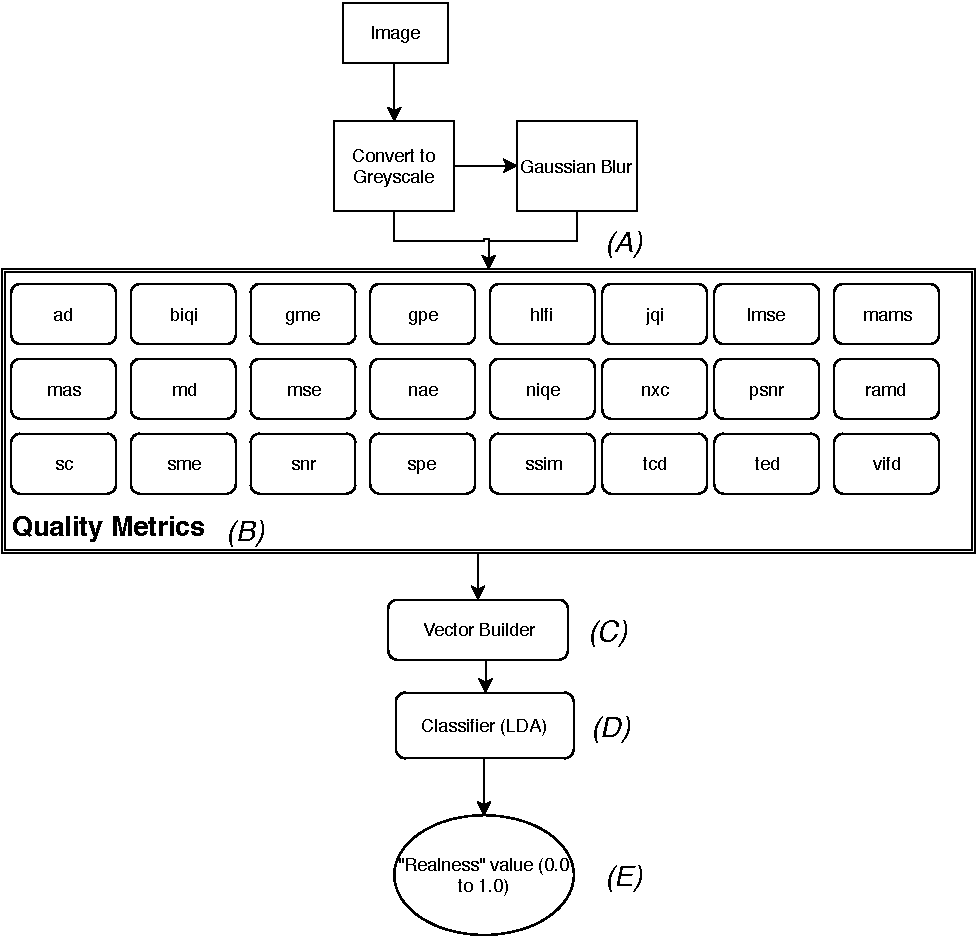
\includegraphics[width=300px]{ImageQualityLivenessTest.pdf}
                \caption{The architecture of the image quality liveness test. (A) The greyscale copy of the image, and a blurred copy of the image are input into each of the metrics.
                (B) The metrics are individually calculated, and a single value output from them. (C) These values build a 1D vector. (D) They are classified using an LDA classifier. (E) The realness value
                is 1.0 for real, and 0.0 for fake, or in between.}
                \label{ImageQualityLivenessTestDiagram}
            \end{figure}

            \subsubsection{Overview}
            A common way of detecting liveness is to consider the image quality of the camera input. When a printout/screen is held up to the camera, the facial image
            will have some noticeable differences, specifically in the high frequencies. There might also be some image compression visible in fake images, compared to real ones.
            This is the basis for the method used.

            More specifically, the implementation was based on the work contained in \cite{ImageQualityAssessmentTest}. 24 different image quality metrics were implemented,
            with metric values being used as an input to a classifier. From previous work, it has been shown that this liveness test is accurate (therefore detecting spoofing well), while also being fairly fast to compute in terms of time, meeting \ref{SpecPoint3} and \ref{SpecPoint1}.

            The classifier used for our implementation was Linear Discriminant Analysis (LDA).

            A visual explanation of the method used is shown in Figure \ref{ImageQualityLivenessTestDiagram}.
    
            \subsubsection{The Metrics}
            The original paper proposed that 25 metrics be used to measure quality. However, our implementation used only 24, due to some implementation problems (explained later).

            Each of these metrics required an input image $I$. Non-reference metrics only required $I$, while full-reference metrics required an additional image $I'$. $I' = Gaussian(I)$ in our implementation.
            
            \paragraph{PyVideoQuality Library}
            As part of the implementation process, the Naturalness metric (NIQE) required the use of a pre-trained classifier which didn't exist for Python. As such, it was necessary to modify the existing code.
            The only Python source code available was \cite{VideoQualityOriginal}, which was written for Python 2 and consisted of single Python files that would be difficult to merge into our system.
            As such, the Python 2 code was converted to Python 3 manually and refactored to follow a python package by myself. This new library was shared-alike and is now available on GitHub. \cite{VideoQualityUpdated} This also had a benefit of separating the metric calculation from the liveness test code.
            
            A sample of metrics, with implementation detail, are outlined below.
           
            \paragraph{Blind Image Quality Index (BIQI)}
                BIQI is a no-reference metric. BIQI consists of two steps: the first is to assess image distortion, and the second is to analyze the quality.  Rather like NIQE, there was no existing BIQI library implementation. The metric takes various different features using wavelet functions and fed them into a classifier component. This element itself would be hard to replicate without the correct processing or training data. The training set used for this quality metric was the LIVE IQA dataset. While this dataset is in the public domain, it required permission to access. This would have taken far too long, for such a small piece of the system.

                As such, it was easier to adapt an existing implementation. A version was found on GitHub that utilised Python 2 focused code. This was manually ported to Python 3. \cite{BIQIImplementation} This ported version is available as part of the project implementation.

            \paragraph{Gradient Magnitude Error (GME)}
            GME is a full reference metric, and it calculates the error corresponding to the gradient magnitude between the two images. The gradients $\Delta I$ and $\Delta I'$
            were calculated using a Sobel filter with kernel size 5 in both X and Y directions. In our implementation, the Sobel filter was calculated using the built-in OpenCV functionality.

                Using these gradients, the metric was calculated using the equation $GME(I, I') = Mean((\Delta I - \Delta I')^2)$. In our implementation, Numpy was again used to calculate both the mean and
                also the squared difference.

            \paragraph{Gradient Phase Error (GPE)}
                GPE is a full reference metric, which like GME used the Sobel filter as a basis. Using four different Sobel filters, gradients in the x and y direction for both
                $I$ and $I'$ were calculated. These were $\Delta I_x$, $\Delta I_y$, and $\Delta I'_x$, $\Delta I'_y$.

                Using these direction gradients, $Mag_{I} = Magnitude(\Delta I_x, \Delta I_y)$ and $Mag_{I'} = Magnitude(\Delta I'_x, \Delta I'_y)$ was then calculated using the gradients shown above.

                Using this, the metric was defined as: $GPE(I, I') = Mean((Mag_{I} - Mag_{I'})^2)$.

            \paragraph{High Low Frequency Index (HLFI)}
                This considers the frequency of specific low and high frequencies within a single image. It is therefore classed as a no-reference metric.
                First, the image was fed through a discrete Fourier transform process using OpenCV. The frequency spectrum was then shifted and a final magnitude spectrum calculated using Numpy. This magnitude spectrum was defined as $M(i, j)$, where the shape of M corresponds to the image I.

                Using this spectrum, a sum of the low frequencies, from $(1,1)$ up to $(i_l, j_l)$ was calculated by cycling through each pixel in the spectrum. These two upper constants for
                the low-frequency band was determined with respect to the shape of M. Given the shape of M was $(X, Y)$, it can be stated that $i_l = 0.15 \cdot X$ and $j_l = 0.15 \cdot Y$.
                For each location (i, j) within the limits, the magnitude spectrum was summed to produce a final value called $lfs$ which was the low-frequency sum.

                A similar process is followed for the high frequency spectrum. However, instead of starting at 1, the starting point is $i_h, j_h$, finishing at $(X, Y)$. The constants $i_h$ and $i_l$ were
                calculated in a similar manner to before, only adding one to the result. Therefore $i_h = Ceiling(0.15 \cdot X + 1)$ and $j_h = Ceiling(0.15 \cdot Y + 1)$, where $Ceiling(x)$ rounds
                a value $x$ up to an integer. The high frequency sum $hfs$ was calculated through this process.

                Based on this, the metric can be defined as $HLFI(I, I') = \frac{lfs - hfs}{\sum_{i,j = 1}^{i,j = (X, Y)} |M|}$.
                
            \paragraph{JPEG Quality Index (JQI)}
                The JQI quality index is used to understand the nature of JPEG compression in an image, specifically with regards to JPEG images being blocky (caused by DCT based compression),
                and blurring components (due to high-frequency DCT coefficients being lost).

                This measures blockiness features (average differences across boundaries), average absolute difference between block samples, and zero crossing rate (where signal changes from positive to negative). 
                These features are combined together to yield an index measuring JPEG quality. The implementation guide followed can be found in the paper \cite{JQIPaper}.
            
                \paragraph{Laplacian Mean Squared Metric (LMSE)}
                LMSE is a full reference metric that considers the edge differences to measure quality. A high LMSE value implies that the input image is of poor quality. 
                    
                This requires a Laplacian function, which is defined in \cite{LMSEPaper} as:

                $$Laplacian(I(m, n)) = I(m+1, n) + I(m-1, n) + I(m, n+1) + I(m, n-1) - 4\cdot I(m, n)$$

                This function is calculated for each pixel location $(m, n)$ in an image. The current implementation uses the Laplacian function defined above, written in Numpy, to produce the Laplacian output. 
                \cite{LMSEPaper}

                Once this operator has been defined, it can then be used to calculate the overall metric: 

                $$LMSE(I, I') = \frac{\sum (Laplacian(I) - Laplacian(I'))^2}{\sum Laplacian(I)^2}$$
                
            \paragraph{Mean Angle Magnitude Similarity (MAMS)}
            LMSE is a full reference metric that considers the edge differences to measure quality. A high LMSE value implies that the input image is of poor quality. 
                
            This requires a Laplacian function, which is defined in \cite{LMSEPaper} as:

            $$Laplacian(I(m, n)) = I(m+1, n) + I(m-1, n) + I(m, n+1) + I(m, n-1) - 4\cdot I(m, n)$$

            This function was calculated for each pixel location $(m, n)$ in an image. The project implementation used the Laplacian function defined above, written in Numpy, to produce the Laplacian output. 
            \cite{LMSEPaper}

            Once this operator had been defined, it was then used to determine the overall metric value, using the equation below:

            $$MAMS(I, I') = \frac{\sum (Laplacian(I) - Laplacian(I'))^2}{\sum Laplacian(I)^2}$$

            \paragraph{Mean Angle Similarity (MAS)}
            This metric is almost identical to MAMS, being a full reference metric that considers the similarity of the angles. Unlike the above, the magnitude of the angles is not considered.

            Using the calculations from the MAMS metric, only the steps up to and including the calculation of $\alpha$ are necessary. 

            Then, MAS can be defined as $MAS(I, I') = 1.0 - Mean(\alpha)$.

            \paragraph{R-Averaged Metric (RAMD)}
                RAMD is a full reference metric, which calculates the average of all differences that are smaller than a specific value $R$.
                In our implementation, $R=10$.

                We create a matrix $D = |I - I'|$.

                With this, this function can be expressed: $$RAMD(I, I') = \frac{\sum_{D(x, y) <= R}^{(M, N)}(D(x, y))}{R}$$

                In the above definition, $(M, N)$ is the shape of both $I$ and $I'$. $(x, y)$ is defined as the coordinates of each pixel. For this calculation,
                the difference is calculated for each pixel location, with any value that's greater than $R$ being set to zero. Then, the remaining values are divided by R.

            \paragraph{Spectral Magnitude Error (SME)}
                SME metric is a full reference metric that utilizes Discrete Fourier Transform (DFT) to analyze the frequency.
                Implementation was achieved using OpenCV and Numpy.

                For image $I$ and $I'$ respectively, a transformed magnitude $M$ and $M'$ is generated using Fourier transform shifts.
                The x component is the real plane, while the y component is the complex plane.

                The metric then follows: $SME(I, I') = Mean((M - M')^2)$.
             
            \paragraph{Spectral Phase Error (SPE)}
                The SPE metric utilizes DFT based transformations which were implemented using OpenCV, with Numpy being used to provide the Fourier transform shift functionality.

                This aims to measure the error within the phase difference between the real and complex planes. Spectral magnitude is calculated using shifts in Fourier transforms,
                for both $I$ and $I'$. Then, the metric follows: $SPE(I, I') = Mean((Magnitude(I) - Magnitude(I'))^2)$.


            \paragraph{Total Corner Difference (TCD)}
                TCD is a full reference based metric. An OpenCV based Harris Detector is used to count the number of corners within each image,
                to yield two values $CornersInI$, and $CornersInI'$. The max number of corners between these images is also found and stored in $MaxCorners$.
                Then, $TCD(I,I') = |CornersInI - CornersInI'| / MaxCorners$.
                
            \paragraph{Total Edge Difference (TED)}
                TED is a full reference based metric. A Sobel filter (using OpenCV) is calculated for both $I$ and $I'$. The absolute difference of this edge map is taken,
                and the mean value is yielded.
                $$TED(I, I') = Mean(|Sobel(I) - Sobel(I')|)$$

            \paragraph{Visual Information Fidelity (VIFD)}
                VIFD is a full reference based metric that considers the quality at 5 different scales. The number of scales can be variable, but in our instance 5 was chosen.
                This method is based on natural scene statistics and is a better indication of how the human visual system measures quality.
                This was implemented into our system using the custom \emph{PyVideoQuality} library outlined above.

            \paragraph{The other metrics used}
                In addition to the above metrics, Absolute Difference (AD), Maximum Difference (MD), Mean Squared Error (MSE), Normalized Absolute Error NAE), Structural Content (SC),
                Peak Signal to Noise Ratio (PSNR) and Signal to Noise Ratio (SNR) were also used. These are full reference metrics, implemented using
                Numpy functionality. The process followed for each metric was defined in \cite{ImageQualityAssessmentTest}.

                The Structural Similarity Metric (SSIM) is a full-reference human perception based model. This was calculated using a \emph{skimage} library function called \emph{compare\_ssim}. 

                The Naturalness Estimator (NIQE) was calculated using the newly completed PyVideoQuality library (explained above).

            \paragraph{The RRED Problem}
            One of the metrics proposed in \cite{ImageQualityAssessmentTest}, Reduced Reference Entropic Distance metric (RRED), was problematic to implement due to the lack of Python implementation available.
            The only implementation available was written in Matlab and relied on Matlab only libraries. While some had Python equivalents, the steerable pyramid functions did not have a Python equivalent, therefore increasing the workload massively for this single metric. Therefore, the metric was ignored for the W-IQA
            test, since the test performance without the RRED metric was within the expected range. 
            
            \paragraph{Testing these metrics}
            Once these metrics were produced, testing was required to ensure these metrics were outputting sensible values that could be relied on.
            Two images were selected at random from the NUAA dataset (using the full image path, rather than the dataset manager created beforehand). These metrics were then carried out individually on these two images. The values were then compared, to see if they differed, and to detect any potential image quality difference. 
            Testing the metrics was slightly challenging as no ground truth data for each metric existed, but viewing the metric values provided a manual testing process.


        \subsubsection{Classifier}
            Initially, a support vector machine (SVM) was used as the base classifier for this liveness test. Grid search was applied to find optimal parameters for the SVM, but despite this, the performance was unreliable. The best SVM results yielded only 70\% accuracy when training and testing on the same dataset, a rather poor result compared to the original paper \cite{ImageQualityAssessmentTest}. Therefore, the classifier was quickly switched to use Linear Discriminant Analysis (LDA), which provided far better performance. This was the classifier specified in \cite{ImageQualityAssessmentTest}.

            For both classifiers, existing SVM and LDA implementations from the \emph{sci-kit learn} Python library were used for their performance. 
            
            The default sklearn LDA settings was initially used, but the results produced still weren't ideal. By using an eigenvector-based solver, and automatic shrinkage, the LDA model performed far better, yielding the results
            shown in the results section.

            Once a model was trained, it needed to be saved for future use. Saving was achieved using the Python \emph{pickle} package. For small models, pickle is ideal since it produces a Python object that can be loaded/written without additional boilerplate. Since the sci-kit learn classifier models don't contain a deep object structure, pickle easily writes the object without recursion issues. With later, larger models (neural network based), pickle wasn't acceptable as Python's version depth limit was reached.
    
            
        \subsection{2D based CNN Liveness Test}
            \subsubsection{Overview}
            As discussed earlier in the paper, there are several different models available for image classification. Unlike ImageNet based classifiers, there are only 2 output classes, which are \emph{real} and \emph{fake}.
            Therefore, the final layer of the model would be different from an ImageNet classifier, but the remaining details would be identical. Unlike the image quality metric, this metric concerns itself with the facial data, to understand which faces
            are real, and which ones are fake.

            \subsubsection{Data Preprocessing}
            \begin{wrapfigure}{r}{100px}
                \centering
                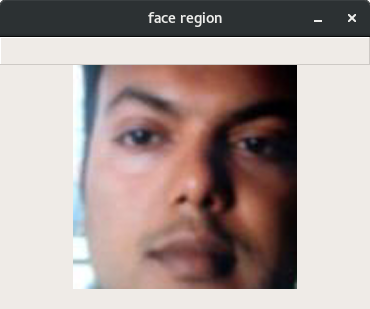
\includegraphics[width=100px]{FaceExtraction.png}
                \caption{This is the output produced from the preprocessing step of the ResNet based method.}
                \label{FaceExtraction}
            \end{wrapfigure}
            
            As this liveness test concerned itself with facial structure, it became necessary to isolate the face from the input image. Furthermore, as part of the CNN model, a required input size was needed to be specified. 
            The preprocessing step, therefore, needed to produce a facial image that had fixed dimensions.

            This was achieved using the \emph{face\_recognition} package. Using this package, a set of bounding boxes of faces is yielded. The largest bounding box (by area) is found, which is taken as the location of the face. Initially, the bounding box was simply cropped and resized to be a square, regardless of its shape. This yielded very poor results  since the dimensions might have been rectangular, yielding the model to incorrectly learn spatial data. As a result, a new method of face isolation based on bounding boxes was designed:
            
            Given a bounding box $B = (top, bottom, left, right)$, a new bounding box $B'$ which has square dimensions can be created by finding the square
            side width $s$. Mathematically, this is defined as:

                $$s = Max(bottom - top, right - left)$$


                The new bounding box can be defined as:


                $$B' = (top, top + s, left, right + s)$$


                By following this method, the model appeared to perform better overall, and produced non-skewed images.

                However, simply isolating the face isn't enough. A fixed size image was needed, in order to be fed into the network. After much experimentation, an image size of $(224, 224)$
                was decided, as smaller dimensions failed to produce adequate results. The resizing was completed using OpenCV. The output of this step is shown in Figure \ref{FaceExtraction}.

                
            \subsubsection{The Model}
               


                \paragraph{Early attempts with AlexNet}
                Initially, an AlexNet based classifier was designed. While AlexNet performance on the ImageNet dataset isn't as high as other models, it provided an ideal starting point to understand the difficulty of the classification. It was eventually found that AlexNet performed relatively poorly on facial liveness classification, and therefore a switch was made to a more complex and better-performing model.

                \paragraph{Residual Networks}
                Residual Networks were chosen over VGG and Inception due to their better performance on ImageNet, coupled with their ability to be easily deployed without excessive memory/computation requirements.
                A ResNet 50 architecture was decided upon, as 50 layers seemed reasonable in terms of the available computational power that was available for this proof of concept. It was deemed that if ResNet 50 works, then ResNet 101 might perform equally, if not slightly better. A ResNet 50 architecture acts as an ideal proof of concept.

                While training a model from scratch might have advantages for some applications, a pre-trained ResNet50 model from the Keras standard library was used. This was done due to work with the small amount of training data available, and also to save time learning the basic features that are present in all generic image classification models. Furthermore, training the entire ResNet50 model would require a large number of parameters to be adjusted, so to further reduce the complexity of the training process, only the last layer was set to trainable, with the other layers remaining static. This method also reduced the risk of overfitting, since there were fewer parameters that required training. This was beneficial due to the small amount of data available from liveness datasets.

                \paragraph{Feed Forward Classifier}
                While a CNN is ideal for processing images, a fully convolutional approach to classification didn't seem appropriate. The output from the ResNet 50 model was flattened and fed directly into a feed-forward neural network.
                While pooling layers were considered, these only take the maximum/minimum/average of specific sections, reducing the dimensionality, and the loss of data means the feed-forward layer has less information to act upon. Therefore,
                it was instead decided to use no pooling layers. The output from the ResNet is flattened and fed into an 8 layer feed forward neural network directly. The first layer of this network has a very large number of nodes,
                while the number of nodes is reduced towards the network output.
                
                \begin{wrapfigure}{r}{180px}
                    \centering
                    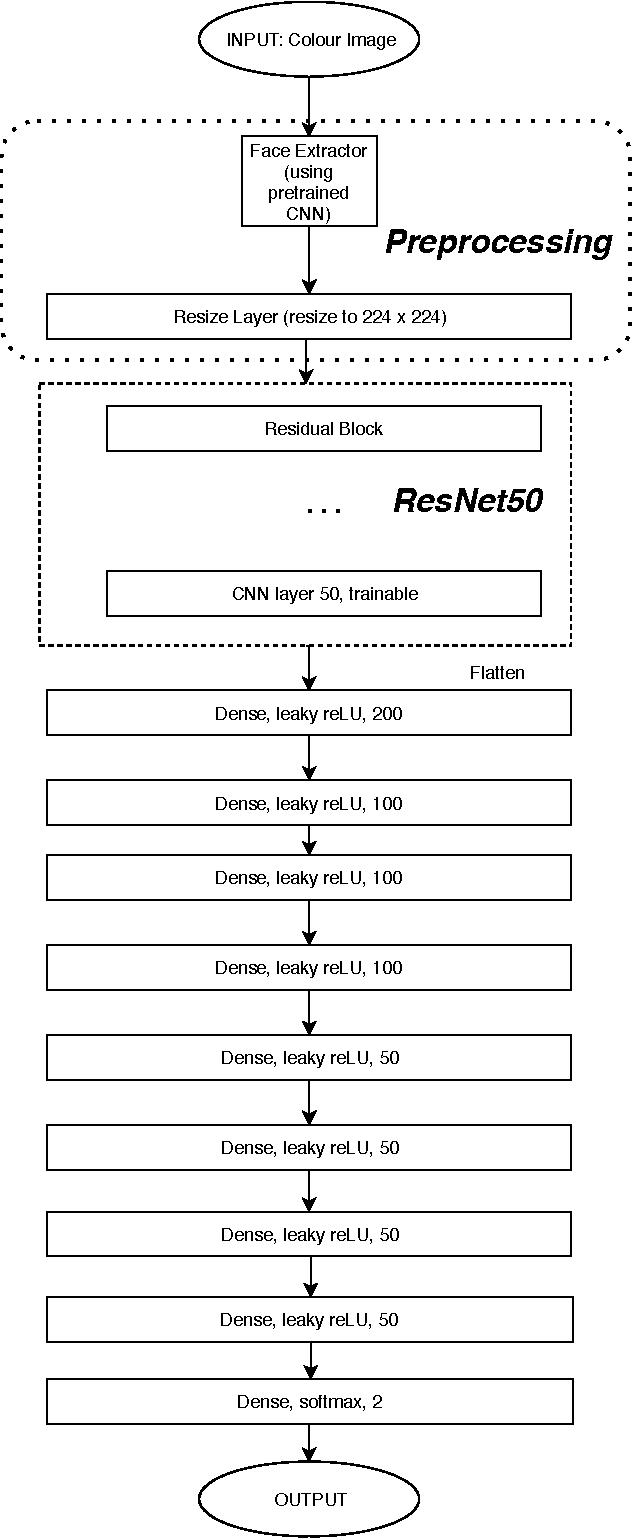
\includegraphics[width=180px]{2DCNNArchitecture.pdf}
                    \caption{The 2D CNN test architecture. We take the face image, resize to a fixed size, and put through ResNet50. The two last CNN layers
                    of this ResNet are trainable. The output of this network is flattened and fed through a deep feed forward network, yielding one output (which is the
                    liveness score as before).}
                    \label{2DCNNArchitecture}
                \end{wrapfigure}
                
                With the initial experiment, the output layer consisted of a single node, with a sigmoid activation function. The entire network was trained using a binary cross-entropy loss function. The network accuracy yielded was fairly reasonable,
                but the confusion matrix showed that the model was outputting \emph{0.0} (fake) for each value, no matter the input. This was a problem, as the network wasn't suitably learning the dataset. As a result, three changes were made to solve the problem, which are outlined below.
                
                \paragraph{The Problem with Activation Functions}
                Initially, the \emph{reLU} activation function was used on all internal nodes within the feed-forward network component. While reLU is very popular for improved speed over traditional activation functions such as hyperbolic tangent and sigmoid,
                for negative values it has a problem. ReLU is positive for all positive values, but 0 for all negative values.

                While all inputs were non-negative, weights could lead to these values becoming negative. There is a known problem called \emph{dying ReLU}, where some neurons output 0
                due to having a negative input (the weights and inputs for all input neurons sum to a non-positive value). Therefore, the model was able to learn 0 (fake) easily, but couldn't learn real (1.0) at all. \cite{liu_liu_2017}

                This problem was counteracted by changing activation function from reLU to Leaky ReLU. Unlike reLU, leaky reLU isn't zero when negative. It requires an input value of $\alpha$, which is used as the gradient of the line when less than zero. \cite{liu_liu_2017} For this model, $\alpha=0.3$. The activation function is defined formally as:
                
                
                \begin{equation}
                    Activation(x) =
                    \begin{cases}
                    x, & \text{if}\ x>0 \\
                    \alpha \cdot x, & \text{otherwise}
                    \end{cases}
                \end{equation}

                \paragraph{The Problem with a Single Neuron Output}
                In order to mitigate the problem of the model outputting zero for each input, the output encoding method was changed. Instead of a single neuron, giving a realness value, two neurons were used.
                These neurons would use the softmax activation function, rather than the sigmoid activation function, to ensure the sum of the neuron outputs would be one (therefore giving a probability that can be used).
                The use of two neurons to encode the realness suggested that the nature for a network to learn 0 is slightly reduced since at least one of the neurons in the output layer must output 1. The encoding method used here
                is called known as one-hot encoding.

                \paragraph{Normalization and Dropout}
                Batch Normalization and dropout were both used within the feed-forward network component to improve learning and to reduce the risk of overfitting. Overfitting was a concern due to the small dataset that was used for training.
                Batch Normalization layers were added between each dense layer, which resulted in increased accuracy of the model.

                Throughout the experimentation process, the model was found to be overfitting. Therefore dropout was added (with a dropout level of 0.3) between each dense layer. This reduced the effects of overfitting.

                The overall outcome is shown in Figure \ref{2DCNNArchitecture}. The normalization and dropout are not visible in the diagram since they are only used for training.

        
            \subsubsection{The Training Process}
                \paragraph{Optimizer}
                Initially, the Standard Gradient Descent (SGD) was used as the optimizer. This was chosen due to the findings of \cite{SGDBetterThanAdamForImageClassification},
                which advised that SGD was better than the Adam optimizer for producing models that generalize. However, after experimenting further the Adam optimizer appeared to generalize better for this project. Using the SGD optimizer, the validation accuracy fluctuated with fairly poor accuracy results overall. The Adam optimizer didn't fluctuate, and the accuracy yielded was much higher.

                It's possible that SGD might perform better over longer periods of time with a very small learning rate, but for small time intervals, Adam appeared to perform better.


                \paragraph{Loss Function}
                Initially, while the model had a single neuron output, the binary cross entropy loss function was used as it's suitable for a single binary output.
                However, when the two neuron output model was introduced, the loss function was changed to use categorical cross-entropy as this was the most suitable
                for a categorical one hot encoding method.

                \paragraph{Data Generators}
                Due to a large amount of data being processed, it was necessary to use a data generator to conduct the preprocessing on the fly. While the preprocessing could have been saved to disc, the preprocessing steps were changed throughout the project making this solution obsolete.

                Initially, Keras' built-in ImageDataGenerator was used, since it allowed for a preprocess function to be passed in. While this worked for a preprocess function that yields the same shape image
                as was input, Keras' ImageDataGenerator does not support resizing images within the preprocess function (e.g. for cropping).

                One solution was to use a Lambda expression within the network to resize the image, but this led to problems with saving/loading models (due to Tensorflow being necessary).

                Therefore, the final solution was to implement a custom generator to manually load images and preprocess them on the fly. This required extending the Sequence class within Keras to produce a Numpy array of data (with the size being the batch size specified). With this new generator, it wasn't necessary to follow this size constraint within the preprocess function. 


    \subsection{3D Face Reconstruction Liveness Test}
        \subsubsection{Overview}
        While 2D methods work well for traditional paper/screen based attacks, they are not designed for detecting the wearing of 3D masks. With 3D printing
        becoming more common, and automatic mask generators also becoming available online, this type of attack is becoming more common.

        The method proposed merged recent developments in facial reconstruction with recent deep learning models for classifying 3D data, to investigate a proposed architecture for a 3D classifier. Unlike previous methods, face data is captured in 2D using a standard device camera, before being reconstructed and then classified.

        \subsubsection{Preprocessing Part 1: Extracting Facial Data}
            This process used the functions from the 2D liveness test, with the face region image being resized to 192x192 (compared to the 224x224 size used by the 2D CNN).
            The same process was followed as outlined previously.

        \subsubsection{3D Facial Reconstruction}
        \begin{wrapfigure}{r}{300px}
            \centering
            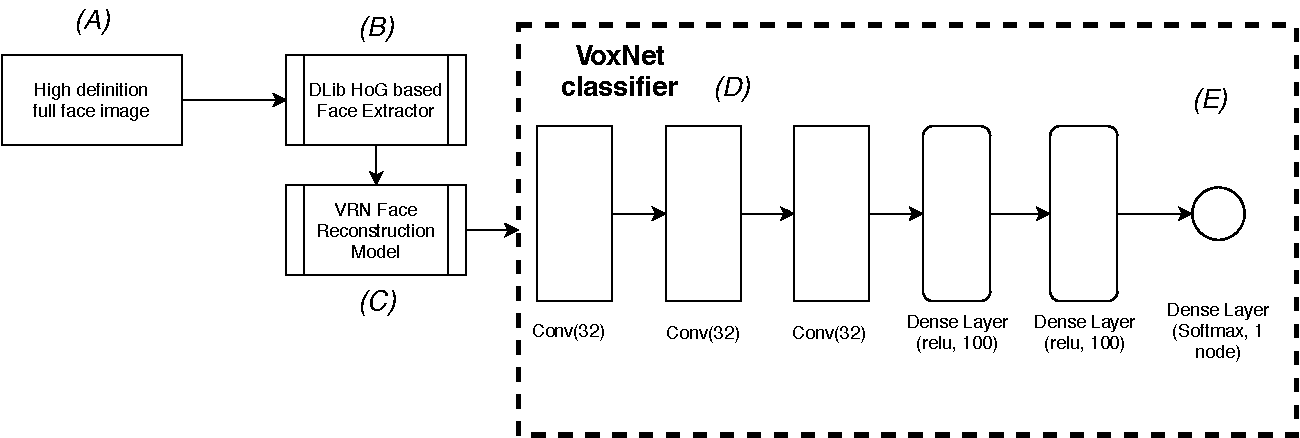
\includegraphics[width=300px]{voxnet.pdf}
            \caption{
                This is an overview of the 3D classifier. \textbf{(A)} a high resolution image is input into the classifier \textbf{(B)} Preprocessing (facial extraction, and resize to 192x192)
                \textbf{(C)} 2D to 3D reconstruction
                \textbf{(D)} Conv3D layers along with feed-forward layers, used for learning the classification
                \textbf{(E)} A single realness metric is output, 1.0 implies real, while 0.0 implies spoofing has occurred.
            }
            \label{3DClassifierArchitectureDiagram}
        \end{wrapfigure}

            A method of obtaining facial structure from a 2D image was required. The VRN method explained in the related work section was chosen. \cite{3DReconstructionMethod}
            While the original work on the reconstruction model used Torch, a version had been previously ported to Keras.\cite{VRNTorchToKeras} This pretrained model took an image of size 192x192, producing a 3D voxel-based representation. 

            In order to correctly modularize the system, the \emph{FaceVoxelBuilder} class was produced to correctly load the pre-trained model, and build the voxel structure for either a single image or multiple images (in the case of batch training).

            While implementing this component of the system, there was a problem: Tensorflow didn't build the objects from the pre-trained model correctly in some cases, as certain components of the model didn't exist on the graph. This was solved by manually creating the predict function by calling a private helper function (\emph{model.\_make\_predict\_function()}).
            This was a known issue with the version of Keras that was being used, and the solution found was specified by the developers of the framework. \cite{KerasVoxNetBug}

        \subsubsection{3D Classification}
            A VoxNet based classifier was chosen, based on the reasonable performance both computationally as well as accuracy wise. 
            While this model can definitely be improved upon, the classifier was believed to produce results that could show a proof of concept,
            and determine whether this method would be suitable for a web-based liveness system. This model was slightly adapted to
            take in a voxel representation of dimensions 192x192x200, higher than the 32x32x32 size used in the original VoxNet paper.
            A deeper feed-forward network was also added to improve prediction performance.
            The final architecture used can be seen in Figure \ref{3DClassifierArchitectureDiagram}.

         

        \subsubsection{The Training Process}
            Training was conducted using a binary cross-entropy loss function, with an Adam based optimizer. Binary cross entropy was used since there was only a single output node,
            compared with a categorical approach. 


            In order to conduct training, a Data Generator was used to minimize memory constraints, since the entire dataset didn't need to be loaded into memory after being preprocessed. Instead,
            only a single batch would be preprocessed on the fly, thus reducing memory usage considerably. Once again, the Keras ImageDataGenerator could not produce 3D output, and therefore
            the custom generator was again used with a preprocess function, this time to produce a 3D output given a 2D image. The code was reused from the previous liveness test for this.

        \subsubsection{The Dataset}
            Unlike the previous two liveness tests, this liveness test relied on a completely different dataset, the Mask Attack Dataset (MAD). \cite{3DMadDataset}

            Since only one dataset was available, cross validation wasn't possible. Therefore, the dataset was divided into a training and test set, separated by subject.

            Subjects 1,2,3,4,5,6,7 were used for training purposes, and 8,9,10,11,12, 13 were used for testing purposes. Splitting up the dataset in this way was necessary to correctly assess the classifier,
            to ensure results give a true indication of how well the model learned the features, rather than how well the model learned the dataset.

    \subsection{Consolidation Layer}
        Each liveness test individually might have some degree of error. Merging the results of each metric together into some classifier to produce a more reliable outcome would be ideal.
        While probability based methods (such as Bayesian calculations) would be feasible, this only works for a larger number of liveness tests. In some cases, very few liveness tests (minimum 2)
        might be used. 

        The solution proposed is to use a classifier, pretrained with the results yielded from the previous liveness tests. After training, this consolidation classifier would be able to spot patterns
        between each liveness test, and hopefully yield a better result by fusing the results of each individual test together. 
        
        In a similar process to the Image Quality Assessment method, an LDA classifier was used with an eigenvector-solver. This was chosen due to the high performance within \cite{ImageQualityAssessmentTest},
        coupled with better performance of the classifier compared to a Perceptron (which can only model linear functions, which might not necessarily be the case with more than 2 liveness tests).
  
\section{Results}
    % based on the solution, what results did we yield? What did we find out?
    For both liveness tests, cross-dataset validation/testing was conducted. Each model was trained using the entire NUAA dataset, and the Replay-Attack test set
    was used to measure the results shown below. In order to visualize the result as a demonstration, a script was written using OpenCV to produce an overlay on top of the image.
    The results of these models in a faux-production environment can be seen in Figure \ref{SystemWorkingScreenshots}. 
    \setlength{\tabcolsep}{2pt}
    \begin{table}[h]
    \begin{subtable}[h]{0.4\textwidth}
        \centering
        \begin{tabular}[t]{lcc}
            \toprule
             & \textbf{W-IQA Test} & \textbf{2D CNN Test}\\
             \midrule
            \textbf{Accuracy (\%)} & 87.0 & 71.2\\
            \midrule
            \textbf{True Negatives (\%)} & 37.5 & 71.5\\
            \textbf{False Positives (\%)} & 12.5 & 1.37\\
            \textbf{False Negatives (\%)} & 0.5 & 22.5\\
            \textbf{True Positives (\%)} & 49.5 & 4.69\\
            \bottomrule
        \end{tabular}
        \caption{Table of results, showing test accuracy with the percentage of test results falling into the specific category defined in the confusion matrix (obtained using sklearn).}
        \label{ResultsTable}
    \end{subtable}
    \hfill
    \begin{subtable}[h]{0.5\textwidth}
        \centering
        \begin{tabular}[t]{lcc}
            \toprule
             & \textbf{W-IQA Test} & \textbf{2D CNN Test}\\
             \midrule
            \textbf{Load time (s)} & 0.00104 & 7.44\\
            \textbf{Time to classify 1 image (s)} & 1.40 & 1.04\\
            \bottomrule
        \end{tabular}
        \caption{Table of results, showing the wall clock time for the load and predict phases of both liveness tests.}
        \label{WallClockResultsTime}
    \end{subtable}
    \caption{Tables showing all numerical results recorded for the two liveness tests.}
    \label{TableOfResultsAll}
\end{table}

    \begin{figure}
        \centering
        \caption{Outputs from the \emph{live\_webcam\_output.py} file, being run on two different videos from the Replay-Attack test dataset. The model predicted the correct output here.}
        \label{SystemWorkingScreenshots}
        \begin{subfigure}[t]{.4\textwidth}
            \centering
            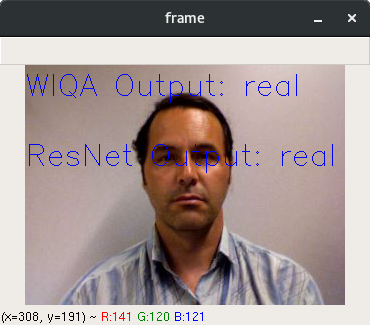
\includegraphics[width=.5\linewidth]{BothRealAndCorrect.png}
            \caption{The system correctly predicting a real piece of data. Image is from a video in the Replay-Attack test dataset.}
            \label{RealScreenshot}
        \end{subfigure}
        \hfill
        \begin{subfigure}[t]{.4\textwidth}
            \centering
            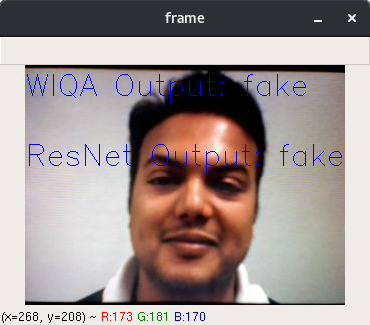
\includegraphics[width=.5\linewidth]{FakeOutputAndCorrect.png}
            \caption{The system correctly predicting spoofing in the input video. Image is from a video in the Replay-Attack test dataset.}
            \label{FakeScreenshot}
        \end{subfigure}
           
   \end{figure}
    \subsection{Testing Process}
        \subsubsection{Datasets}
            The Replay-Attack test dataset was used to access the results of each liveness test. This dataset contains no overlap with the set that was trained on, therefore ensuring that
            the results are a true indication of the generalised performance.

        \subsubsection{Accuracy}
             Top-1 accuracy is an ideal metric to judge the performance of the system since a high Top-1 accuracy in the results would show how often the liveness test yields the correct results.
            
            A Top-1 accuracy figure of 50\% implies that the model is simply randomly yielding output (since there are two cases), which isn't ideal. A figure of 70\% implies that the model is reasonably returning the correct result and is feasible, but might need minor changes or more training to yield a better result. A figure of over 85\% implies that the model is producing the correct results most of the time. The higher the accuracy figure, the better, when being run on an unseen dataset.

        \subsubsection{Confusion Matrix}
            While accuracy is a reasonable metric, it's also important to visualize how often each model selects each case (fake/real), and whether the selection is correct or incorrect.
            There are four important terms with the confusion matrix. These are:
            \begin{multicols}{2}

            \paragraph{True Positives}
                This is the percentage where the model predicts that a given input is real, where the input is indeed real. Therefore, the liveness test has identified a user as real correctly.
                This figure should be above zero, and a reasonable figure. 

            \paragraph{False Positives}
                This is the percentage where a model predicts an input is real, where the input actually contains a spoofing attack. This is a concern since for security-focused
                liveness test, this should be mitigated as much as possible.

            \paragraph{True Negatives}
                This is the percentage where a model predicts an input is fake, where the input contains a spoofed image. This is an indication of how often a model predicts that an input is faked.
                This again should be reasonably high.

            \paragraph{False Negatives}
                This is the percentage where a model predicts an input is fake where it's actually real. This isn't ideal, but this is the preferred option when a liveness test performs poorly, since
                this would only cause inconvenience for the user, rather than a potential security breach.
            \end{multicols}
   
    % CNN table: 4317 & 83 & 1357 & 283
    \subsection{Image Quality Liveness Test}
        Overall, the Image Quality Test performed as expected with reference to the initial paper.\cite{ImageQualityAssessmentTest}
        The overall results, shown in Table \ref{ResultsTable} show fairly good performance on the Replay-Attack test dataset, with an accuracy of 87\%. While accuracy gives an overall account of the results, it doesn't show the overall performance.
        
        The level of true negatives and true positives respectively are fairly high, but the number of false positives was slightly higher than expected.
        What's interesting to note is the low number of false negatives which in our security-conscious case isn't desired (since inconvenience isn't as much of a problem as security).
        However, the overall performance was better than anticipated.
        % Total results - the RAW data in case people need it.
        % 0.87
        % True Negatives:  75
        % False Positives:  25
        % False Negatives:  1
        % True Positives:  99
        While accuracy is important, the time taken for the model to classify a single image is also important. The LDA method took 1.40 seconds to classify a single 2D image, which is within the specified 2 seconds bound.
        Also, the model itself is very small and therefore can be loaded in a very minute amount of time (0.001 seconds). The bulk of the time required is in the calculation of the metrics, rather than the classification process,
        and therefore future speed optimizations could consider improving the calculation of the metrics. These results can be seen in Table \ref{WallClockResultsTime}.

    \subsection{2D Convolutional Neural Network Liveness Test}

    The performance of our liveness test can be seen in Table \ref{ResultsTable}. While not as accurate compared to the W-IQA model, this liveness test still detects true negatives with a fairly high percentage.
    While the accuracy of this model could be improved with further training or by deepening, the results show that this basic architecture is feasible. In the security alert environment of facial liveness,
    false negatives, while potentially annoying to the end user, are an ideal result compared to false positives (which would imply that someone is real when they are fake). While false positives still exist, their number is small compared to the number of negatives.
    Furthermore, the number of positives is small, meaning that this model leans on the side of caution, something that is ideal. Therefore, this model would be secure and accurate enough with further training (and potentially replacing ResNet50 with a deeper ResNet model).

    The time taken to load the model from memory was the main bottleneck in terms of computational performance, as loading the model into memory for the first time took 7.44 seconds. However, once the model was loaded,
    the time taken to predict a single image is very small, on average taking 1.04 seconds, which is even smaller than the W-IQA test, and almost half the specified 2 second time, which is ideal. These results can be seen in Table \ref{WallClockResultsTime}.     
        % Confusion Matrix = [[4317  283]
%           [1357   83]]

    \subsection{3D VoxNet Liveness Test}
    This method had some major performance challenges. The 3D facial reconstruction worked well, producing the desired outcome. However, the 3D classifier (VoxNet), had numerous problems.
    The original VoxNet model, proposed in \cite{VoxNetModel}, used 32 filters for the Conv3D layers (with a 32x32x32 input). However, using 32 filters in our model for each Convolutional Layer (alongside the larger data input than expected),
    led to memory errors and wasn't able to be trained on the training hardware.  Reducing the 3D reconstruction resolution wasn't an option since the entire model would require retraining (which would take lots of time, resources, and wasn't feasible).
    Furthermore, as seen with the 2D CNN method, reducing the resolution might also reduce accuracy. Therefore, the remaining solution was to reduce the number of filters down to a small 12 filters per convolution layer.

    During the training process, with a variety of learning rates, the accuracy of the model didn't leave 50\% with a differing amount of batch sizes. This indicates that the model wasn't learning the features correctly (potentially due to the lack of filters in the Convolutional Layer).
    
    While the classifier itself didn't work and yield any meaningful results, it's also important to consider the time taken for a 2D image to be reconstructed. 
    To reconstruct a single image from 2D to a 3D face structure, it took 5.39 seconds, which already exceeds the 2-second constraint set by the specification.
   
    Due to the poor accuracy with a low number of filters, the excessive amount of memory required for unknown accuracy results, and the large time taken to reconstruct the 3D structure (not including the added time to theoretically classify the result),
    this liveness test clearly isn't feasible for the purpose of a web liveness service.
    
    \subsection{Consolidation Layer}
    \begin{wrapfigure}{r}{230px}
        \centering
        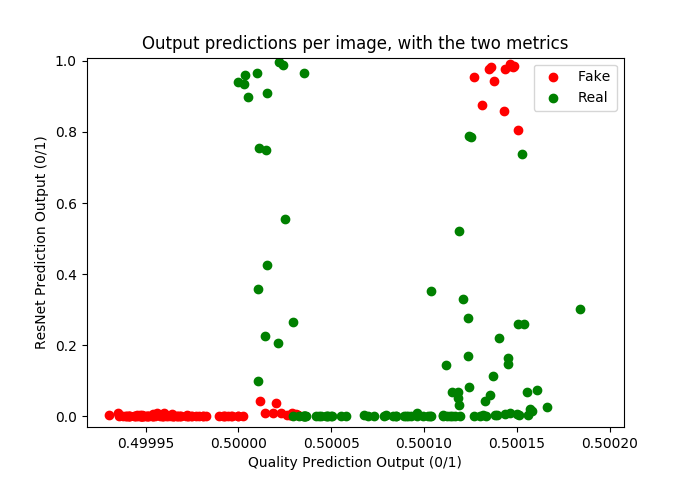
\includegraphics[width=230px]{LinearlySeparable.png}
        \caption{A plot of ResNet output against WIQA output. While a perceptron could be used (due to the linearly separable nature), this would effectively yield a logical AND or OR gate with 2 liveness tests.}
        \label{LinearlySeparableGraph}
    \end{wrapfigure}
  
    
        As shown in Figure \ref{LinearlySeparableGraph}, plotting the results together with the probability outcome (rather than the class outcome),
        yield a plot where the two classes could approximately be divided up with a single line. Therefore, as expected, the relationship between predictions is linearly separable.

        While investigating this further, using an LDA as a consolidation layer yielded fairly ideal results: 75\% accuracy to be precise. 

        However, it's important to note that while this operated for two liveness tests, it could not be tested for a greater number of liveness tests. While accuracy was fairly reasonable,
        using more metrics could yield improved accuracy.

    \subsection{Live Application}
        While numerical figures are useful to measure the results, it's also important to show performance on a completely unseen subject (through the use of a webcam). An OpenCV based script was
        written to, in real time, access the output of the liveness tests and overlay the results on the screen with their predictions. 

        The successful results can be seen in Figure \ref{SystemWorkingScreenshots}. While not numerical, it yielded a large number of useful insights into the real-time nature of such a system,
        and it's practical deployment.

        \begin{multicols}{2}
            \paragraph{Benefits of CNN facial isolation}
            The CNN facial isolation was found to be very good at selecting the facial area ready for preprocessing. Even with part of the face covered up, it still yielded a reasonable
            facial crop, which could then be fed into the network. Also, the head being placed at different angles also yielded a reasonable face isolated image that could be used for the
            CNN metric.
        
            \paragraph{Resolution problems with WIQA test}
                While the test datasets contained a small number of different resolutions, the differences in resolutions were minimal. Therefore, using a completely different image resolution
                of 1280x720, which was completely unseen by the classifier previously, led to the model predicting each input as real, which was incorrect.
    
                The solution taken was to resize this image down to a more reasonable 640x480, which yielded far better performance in real time. However, in future iterations, resolution is
                a factor that needs to be considered, and potentially the resolution should be included in the classified vector. Furthermore, more resolutions should be tested to yield a reasonable
                classification.
    
            \paragraph{Uncertainty of the CNN liveness test}
                While the CNN liveness test could correctly classify a specific facial input, it would occasionally change the prediction to an incorrect prediction
                as frames were stepped through. This was even observed with minimal change in the input image. Since the prediction of 1 image takes minimal time,
                it might be ideal in future to take a set of 8 frames, and output the mode classification from this batch, this way smoothing out the prediction.
                Alternatively, the CNN liveness test might need more training to assert the difference between real/fake in a more varied set of lighting conditions and resolutions.
    
            \paragraph{Problem in running liveness tests in series}
                Since we have two liveness tests, the script runs the WIQA test first, before running the CNN based liveness test. This is fairly slow, as each liveness test requires their
                own resources and time to complete. It might be more ideal to parallelise this in future, to yield better performance. While single-computer parallelisation might not be the best option
                (since each classifier requires some degree of multithreading), multiple systems could be used to speed up this process.
    
        \end{multicols}
      
\section{Evaluation}
    % How well our system works, how well did it assess stuff, and how it can be improved.
    % what are the uses of our research? e.g. influence and improve the design of xyz...
    \subsection{Usefulness of our system}
    
        % Identified two metrics that could be deployed.
        % Created the structure of such a system (e.g. consolidation layer) to allow for future extensions with further liveness tests.
        % Applications: within IoT devices, use within web browsers alongside existing face recognition services. 
        % There is an argument that one could steal your likeness and use it elsewhere on the internet. However, providing liveness tests
        % are suitable, there is no other way of stealing ones face. There would be a need to ensure furhter development of such a system.
        % Developing a single component as a service would mean developers could focus on developing their applications. 
        \paragraph{Quality Test}
            The Quality Test performed well, and is suitable for a web based liveness service due to the high 87\% accuracy achieved.
            True positives and true negatives (that is, correct predictions for both real and fake) were high which means that the classifier
            is classifying correctly. However, the high false positive rate shows a slight cause for concern, since the model in 12.5\% of cases
            classified a fake image as real, which isn't ideal for our security focused solution. This could potentially be solved by adjusting output
            variable of the classifier (using a figure representing 'fakeness' rather than realness). This would hopefully lead to more false negatives,
            which are inconvenient but more secure for the system.

            In terms of computational performance, a 1.40 second time for classifying a single image is within the limits of the expected 2 seconds, and could be improved further
            with parallel based methods, and not relying on libsvm for the BIQI metric.
        \paragraph{2D CNN}
            The 2D CNN Test performed adequately. While the accuracy was lower than expected (at 71\%), the classifier still performed similarly to the accuracy expected on
            ImageNet (since 76\% was yielded with ResNet50 on the ImageNet dataset). This is shown in Figure \ref{Top1AccuracyOverNetwork}.

            True negative classification was high, with a total percentage of 71.5\% of all classifications being true negatives. While the number of false negatives also being fairly high,
            this is preferred to errors being false positives (since in this case, the model yielded a result that doesn't cause a security problem).
            The model showed it could classify true positives, but this figure was fairly low. Incorrect labels during the training process might have been one cause of this,
            since some images could not have any face extracted, and were labelled as either real or fake, despite being outliers. Furthermore, the model might have been
            another factor, since ResNet50 yielded a slightly higher 76\% accuracy when classifying ImageNet, so a larger model might also improve the results in future.

            In terms of performance, classifying an image is very quick, but the time taken to load the model is what took the most time (due to memory needing to be allocated and written to).
            In production, providing a model was preloaded and ready to accept input, the computation time of this metric would be very fast, and therefore be ideal for inclusion in a liveness web service.
        
        \paragraph{3D VoxNet Liveness Test}
            As seen from the results, this method of liveness test isn't feasible. With extra training, while the accuracy of the model could be improved, the
            real time memory requirements don't seem feasible. Based on the VoxNet paper, the accuracy achieved with a 32x32 VoxNet classifier on the SUOD dataset (a 3D dataset of objects)
            is 69\%. While this accuracy could be justified with reasonable computational and memory characteristics, this further proves that this method isn't feasible in the current state. In the future, a new approach of detecting 3D attacks is necessary.
        
    \subsection{Improvements}
    \begin{multicols}{2}
        \paragraph{Representing 3D Attacks}
        While a fully 3D based approach didn't work, a 2D based model could detect elements of spoofing in the 2D image.
        A ResNet based model could be used to detect 3D based attacks, using a similar approach to the 2D CNN used within this project.

        \paragraph{More Liveness Tests}
        While the consolidation layer proposed functioned for 2 liveness tests, introducing more liveness tests within this structure would allow
        analysis of the performance of the proposed LDA consolidation layer at scale.

        \paragraph{Existing BIQI implementation}
            The existing BIQI implementation could be re-implemented using \emph{sklearn} to provide the SVM implementation, rather than the existing \emph{libsvm} executables.
            Porting the existing SVM should be possible.

        \paragraph{Replacing ResNet50 with a larger ResNet model}
        While ResNet50 performed well, utilising a larger ResNet model with more layers (e.g. ResNet101), a higher accuracy could be obtained.
        Larger ResNet models have yielded better accuracy on the ImageNet dataset, and one would therefore expect this to occur with the liveness test too.
    \end{multicols}
\section{Conclusions}
    % overall, what did the project show?
    % TODO this needs to probably be reworded.
    This project showed that creating a facial liveness service for the web is a feasible idea, and performs fairly well for 2D attacks, with adequate accuracy and computational requirements.
    The image quality liveness test is accurate and fast, while the ResNet based method is a feasible idea and performs adequately, and could be adjusted further to improve the accuracy. For 3D attacks however, the
    proposed VoxNet based model performed badly and is not recommended for inclusion in a liveness test web service.

    % In addition, the improvements to the existing system were shown, and potential GDPR considerations were shown on how to implement such a system to better comply with the regulation. In building of a system for commercial use, it's important
    % to note that licensing on training and testing datasets would require new datasets be used.

\printglossary
\bibliographystyle{abbrv}
\bibliography{report}

\end{document}